\chapter{Fundamentos Teóricos}
En este capítulo se describirán aquellos conceptos teóricos fundamentales para comprender el trabajo realizado en este proyecto.

\section{Optimización}
La optimización es un campo de estudio que trata, mediante el uso de las adecuadas herramientas matemáticas, de maximizar o minimizar una función objetivo. Esto significa, obtener la mejor solución posible para un problema dado dentro de un conjunto de alternativas y normalmente sujeto a una serie de restricciones que hacen de una solución satisfacible. Es un área interdisciplinar que aborda desde campos tales como la Economía, Ingeniería, Biología y muchas otras tantas disciplinas.\\[6pt]
La optimización es una disciplina arraigada en la naturaleza humana. Este impulso innato hacia la optimización ha llevado al desarrollo de diversas metodologías y técnicas a lo largo de la historia, desde los rudimentarios métodos de prueba y error hasta los sofisticados algoritmos de optimización computacional utilizados en la actualidad.

\subsection{Definición general de un problema de optimización}
Para poder convertir un problema abstracto en un problema de optimización concreto, con el que se pueda trabajar, es necesario establecer ciertos elementos fundamentales que lo definan de manera precisa y clara. En general, un problema de optimización se expresa de la siguiente forma~\cite{inbook}:

\begin{subequations}
    \begin{alignat}{2}
         & \text{Función objetivo a minimizar}                       & \qquad & f(x)\label{eq:optProb}                             \\
         & \text{Sujeto a} \nonumber                                                                                               \\
         & s \text{ restricciones de desigualdad}                    & \qquad & g_i(x)\leq 0, \quad j=1,2,...,s\label{eq:optProb2} \\
         & w \text{ restricciones de igualdad}                       & \qquad & h_j(x) = 0, \quad j=1,2,...,w\label{eq:optProb3}   \\
         & \text{Donde el número de variables es dado por} \nonumber & \qquad & x_i, \quad i=1,2,...,n
    \end{alignat}
\end{subequations}

La definición general de un problema de optimización proporciona una estructura sólida para abordar el problema abstracto. Establece la función objetivo que se busca minimizar o maximizar, junto con las restricciones que deben cumplirse. Estas restricciones pueden ser tanto desigualdades como igualdades, y todas juntas definen el \textbf{espacio de búsqueda} del problema.

\subsection{Función objetivo y función fitness}
Ambos términos, aunque a menudo se utilizan como sinónimos, desempeñan roles distintos en el ámbito de la optimización. La función \textit{objetivo}, como su nombre indica, establece el objetivo a alcanzar en la resolución del problema. Esta función cuantifica el rendimiento de las soluciones encontradas en relación con el objetivo específico del problema, que puede ser maximizar ganancias, minimizar distancia, entre otros objetivos. Por otro lado, la función de \textit{fitness} solo tiene que evaluar la idoneidad de una solución dentro de una población de soluciones. Es decir, determina la calidad relativa de la solución respecto a otras alternativas.

Por otro lado, la función objetivo puede ser positiva o negativa, dependiendo de si se busca maximizar o minimizar el objetivo. Además, la función \textit{fitness} también puede llegar a ser una aproximación de la función objetivo, pero no necesariamente coinciden exactamente.\\[6pt]
Resumiendo, la función \textit{fitness} es un tipo particular de función objetivo que se utiliza como métrica de rendimiento~\cite{eiben2015}.

\subsection{Óptimos globales o locales}
Se conocen como punto de óptimo global (mínimo o máximo) la solución (o vector hablando en términos matemáticos) cuyo valor para la función objetivo es el más grande o más pequeño en todo el espacio de soluciones posible, es decir, el espacio de búsqueda. Los óptimos locales en cambio son varios, no solo uno como es el global. Son pequeños picos o depresiones a lo largo de la función, los cuales marcan un máximo o mínimo dentro de un vecindario o región de soluciones.

\begin{figure}[htp]
    \begin{center}
        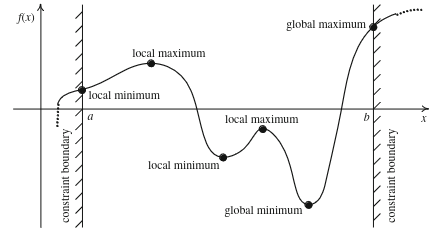
\includegraphics[width=1\textwidth]{imagenes/min-max_points.png}
    \end{center}
    \caption[Puntos globales y locales]{En esta figura extraída de \cite{inbook} puede observarse de manera intuitiva la diferencia entre punto global y puntos locales. El máximo global es el valor más alto para $f(x)$ en el espacio, mientras que un máximo local solo representa el valor más alto dentro de un ``vecindario".}
\end{figure}

Sea $f(x)$ una función a maximizar y $x^*$ una solución óptima. Un objetivo $G(x)$ está en su máximo global sí y solo si~\cite{inbook}:
\begin{equation}
    f(x^*) \geq f(x) \quad \forall x
\end{equation}
En cambio el objetivo está en un máximo local en el punto $x^*$ si:
\begin{equation}
    \begin{split}
        f(x^*) \geq f(x) \quad & \forall x \\
        & \text{dentro de un vecindario de } x^*\text{~\cite{inbook}}
    \end{split}
\end{equation}

\section{Selección de características}
La selección de características es un ejemplo de problema $NP$-Hard y uno de los problemas más importantes en el mundo de la inteligencia artificial, más concretamente en el \textbf{machine learning} o aprendizaje automático.

\subsection{Necesidad y motivo}
El aprendizaje automático se basa en los datos como fuente de aprendizaje. Es indispensable tener un buen conjunto de datos para poder obtener un modelo robusto y preciso. Por norma general o como se diría en inglés \textit{``as a rule of thumb''}, a más grande el conjunto de datos, mayor calidad del modelo. De hecho hay una correlación inmediata con esta sentencia.

\begin{figure}[htp]
    \begin{center}
        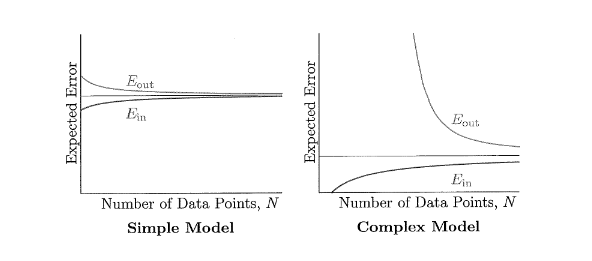
\includegraphics[width=1\textwidth]{imagenes/learning_from_data_vc.png}
    \end{center}
    \caption[Correlación entre error del modelo y N]{Esta figura extraída de \cite{Mostafa2012} visualiza la relación directa entre calidad del modelo (menos error esperado) y número de datos que se le proporciona al algoritmo de aprendizaje.}
    \label{fig:learning_from_data_vc}
\end{figure}

Es inmediato pensar que, a mayor cantidad de datos, mejor calidad del modelo, y así suele ser. Sin embargo, también existe una ``normal general'' que relaciona la complejidad del modelo y su capacidad de generalización. Es cierto que un modelo muy complejo (muchos parámetros) es capaz de ajustar mejor funciones más complejas, pero dentro de un conjunto con una serie de modelos suficientemente complejos, suele ser mejor idea elegir el más simple. Hay una serie clara de ventajas para ello:
\begin{enumerate}
    \item Menor  sensibilidad al sobre-ajuste.
    \item Mayor interpretabilidad del modelo y sus resultados.
    \item Mayor eficiencia y por tanto menor tiempo de ejecución y menor peso en memoria.
\end{enumerate}

De hecho, como puede observarse en la figura \ref{fig:learning_from_data_vc}, el modelo más complejo tiene un error esperado mucho mayor que el simple. El $E_{out}$ o error fuera de la muestra (error de generalización) es mucho más abrupto, es decir, generaliza peor.\\[6pt]
Por supuesto, con suficientes datos, con un $N$ (número de datos) suficientemente grande, la tendencia del error es a la baja~\cite{Mostafa2012, shalev2014understanding}. Ocurre, sin embargo, que la recolección, limpieza y transformación de datos es una tarea compleja, por ello es mejor ceñirse, de nuevo, al modelo más pequeño que obtenga una solución con suficiente calidad.\\[6pt]

Como se ha mencionado anteriormente, la selección de características ayuda a la reducción del ruido. Siendo $f$ la función objetivo a predecir, $H^n$ el conjunto de hipótesis o conjunto de modelos de dimensión $n$ posibles, $h^*(x)$ el mejor modelo aprendido y $x$ una variable de entrada. El ruido conocido
como ruido estocástico es aquel que atiende a una variación aleatoria que
puede surgir de diversos factores, como mediciones imprecisas de señales o la falta de
precisión en sensores. Por otro lado, el ruido determinista está directamente
relacionado con la complejidad de un modelo. Su presencia aumenta la probabilidad de
sobre-ajuste. El ruido determinista puede explicarse como la parte de la función $f$ que el conjunto
de hipótesis $H^n$ no puede capturar, es decir, $f(x) - h^*(x)$. Este tipo de ruido se
considera así porque la función (modelo) no es lo suficientemente compleja como para comprender
esa parte. Este ruido depende de $H^n$ y permanece constante para un valor dado de $x$~\cite{Mostafa2012}.\\[6pt]
La reducción de características ayuda a manejar ambos tipos de ruido~\cite{miao_survey_2016,Mostafa2012} al simplificar el
modelo, lo que puede reducir el impacto del ruido estocástico y disminuir la complejidad del
modelo, lo que a su vez puede ayudar a mitigar el ruido determinista al mejorar la capacidad
del modelo para capturar las características relevantes y descartar las irrelevantes. Una selección adecuada de características puede ayudar a identificar y centrarse en las más informativas, revelando potencialmente los verdaderos patrones subyacentes en los datos, lo que puede reducir el ruido determinista.
Esto puede conducir a una mejor capacidad de generalización y a una reducción del sobre-ajuste.\\[6pt]

\subsection{Concepto}
El funcionamiento y motivo es explicado ya en la sección de motivación en \ref{motivation}. Por evitar redundancias se procede a explicar el concepto de manera abreviada y puntualizando en los apartados más importantes.\\[6pt]
La selección de características es una conocida y necesaria técnica de pre-procesamiento de datos para la construcción de un modelo de aprendizaje. Su función es escoger un subconjunto óptimo de características dentro del conjunto inicial, de forma que la complejidad del modelo se reduzca.\\[6pt]
Este problema es del tipo $NP$-Hard, como ya se ha mencionado previamente en \ref{motivation}.
La selección de características ayuda a una serie de factores como son la interpretabilidad, mejora de la eficiencia temporal y espacial del modelo y sobre todo con la \textbf{maldición de la dimensionalidad}~\cite{venkat2018curse, bellman1957dynamic}.

\subsection{Maldición de la dimensionalidad}
El término fue acuñado por Bellman en $1961$~\cite{bellman1961adaptive}. Este fenómeno ocurre cuando la dimensionalidad de los datos es muy grande. En un espacio de características de alta dimensión, es común que los datos estén muy dispersos, lo que significa que hay muy pocos datos en comparación con la cantidad posible de características. Esto dificulta que los modelos representen correctamente todo el espacio de características~\cite{peng_interpreting_2024}.

\begin{figure}[htp]
    \begin{center}
        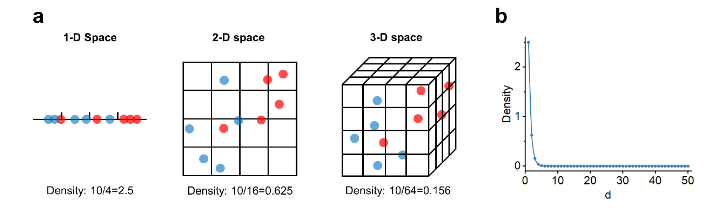
\includegraphics[width=1\textwidth]{imagenes/curse-dimen-example.png}
    \end{center}
    \caption[Tendencia de incremento de dimensionalidad en varios espacios de características]{Esta figura extraída de \cite{peng_interpreting_2024} muestra la tendencia en la densidad a medida que se incrementa la dimensionalidad del espacio. En $(a)$ se muestra la densidad con diez puntos de datos en un espacio $1D$, en $(b)$ se muestra la tendencia al incrementar las dimensiones.}
\end{figure}

Además, en espacios de alta dimensión, la medición de distancias puede volverse menos precisa. Esto se debe a que las distancias entre puntos de datos diferentes tienden a converger a un mismo valor a medida que aumenta la dimensionalidad. Esto significa que las medidas de distancia ya no son tan útiles para medir la similitud entre datos~\cite{peng_interpreting_2024, venkat2018curse}. En el trabajo de Beyer y colaboradores~\cite{beyer99nn} se observó como esto ocurría y por tanto un escaneo lineal (recorrer los puntos uno a uno) resultaba en altas dimensiones más práctico que otras técnicas complejas.
\section{Metaheurísticas}
Dentro de la optimización hay muchos tipos de métodos, dentro de los pseudoaleatorios pueden encontrarse las metaheurísticas. Estas son algoritmos basados en una abstracción de mayor nivel de la \textbf{heurísticas}. Mientras que las heurísticas se apoyan en el conocimiento específico del campo en el que se encuentra el problema, y están restringidas a su dominio, las metaheurísticas son aplicables a todo tipo de problemas, independientemente de su área de optimización~\cite{bianchi2009survey}. Es cierto que hay algoritmos que son más convenientes para ciertos problemas que otros, pero su aplicación es generalizada. Normalmente, las metaheurísticas son diseñadas siguiendo una inspiración en la naturaleza, ya sea en fenómenos físicos o en el comportamiento animal. Ejemplo de estos son algoritmos como el \textit{Búsqueda Cuckoo}, \textit{Enfriamiento Simulado} o incluso \textit{Algoritmos Genéticos}.\\[6pt]
Las metaheurísticas son especialmente útiles en problemas cuya resolución no es factible debido a altos costos computacionales, ya sea porque es posible analíticamente pero computacionalmente costoso, o porque el problema no es abordable mediante algoritmos convencionales. Son capaces de encontrar óptimos locales lo suficientemente aceptables, soluciones no óptimas, pero si muy buenas~\cite{bianchi2009survey}.

\begin{figure}[htp]
    \begin{center}
        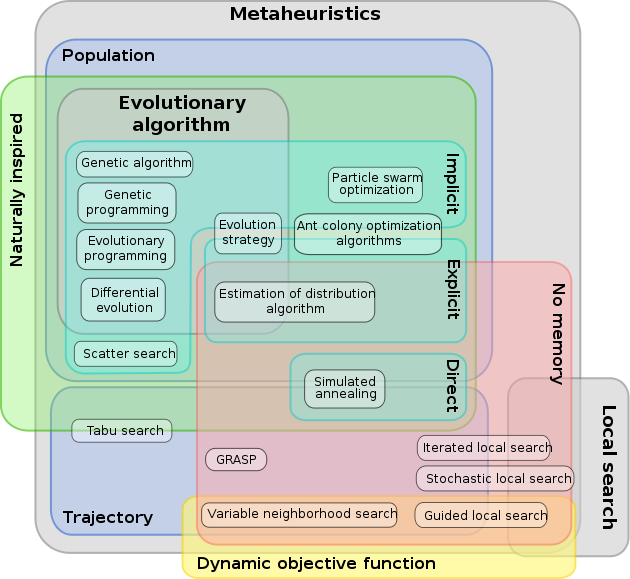
\includegraphics[width=0.8\textwidth]{imagenes/mh_euler_graph.png}
    \end{center}
    \caption[Clasificación metaheurísticas]{En esta figura de los autores Johann ``nojhan'' Dréo y Caner Candan, se clasifican las distintas metaheurísticas por inspiración.}
\end{figure}

\subsection{Exploración vs explotación}
Las metaheurísticas, y algoritmos basados en técnicas pseudoaleatorias, deben tener un balance entre sus factores explorativos y explotativos. De no ser así, los algoritmos tendrían tendencias a la convergencia temprana, dejando de lado mucho espacio por explorar y por ende soluciones posiblemente mejores (estancamiento en óptimos locales) o serían muy lentos en la convergencia hacia una solución.\\[6pt]
La \textbf{exploración} se refiere a la habilidad del algoritmo de buscar nuevas y diversas regiones en el espacio de búsqueda/solución. Es una característica de la búsqueda global, que también puede ser llamada \textit{diversificación}. En cambio, la \textbf{explotación} es la habilidad de la búsqueda de explotar las mejores soluciones encontradas hasta el momento y mejorarlas localmente, dentro de un ``vecindario''~\cite{xu2014exploration}.\\[6pt]
No existe un equilibrio \textit{de facto} entre exploración y explotación en las metaheurísticas. Aún no se ha alcanzado una respuesta definitiva a esta cuestión. Desde una perspectiva de sistemas, una metaheurística puede entenderse como un sistema dinámico compuesto por numerosos ``individuos'' que interactúan entre sí. Estos individuos representan las distintas soluciones o posiciones en el espacio de búsqueda que la metaheurística explora~\cite{6896450}. Las interacciones entre estos individuos son las que conforman comportamientos explorativos o explotativos y dependen del problema a solucionar y del propio algoritmo su equilibrio.

\section{Teorema No Free Lunch}\label{sec:teorema-no-free-lunch}
El Teorema de ``No Free Lunch'' (NFL) establece que, en promedio, ningún algoritmo de búsqueda puede superar a otros algoritmos en la búsqueda de todas las funciones objetivo posibles. En otras palabras, no existe un algoritmo universalmente óptimo que pueda dominar en todos los problemas de búsqueda. Esto implica que, si un algoritmo es efectivo para un conjunto particular de problemas, es probable que no lo sea para otros~\cite{585893}.\\[6pt]
Relacionar este teorema con las metaheurísticas implica reconocer que no hay una única metaheurística que sea la mejor para todos los problemas de optimización. Cada problema puede tener características únicas que lo hacen más o menos adecuado para ciertas metaheurísticas. Por lo tanto, en lugar de buscar una solución universal, las metaheurísticas se centran en explorar y explotar diferentes áreas del espacio de búsqueda para encontrar soluciones aceptables o incluso óptimas para problemas específicos.\\[6pt]
Pese a ello, las suposiciones de este tipo de teoremas, como conjuntos de datos extraídos de una distribución uniforme sobre todos los conjuntos de datos posibles, están completamente desalineadas con el mundo real, donde los datos suelen ser altamente estructurados y no están uniformemente muestreados~\cite{goldblum2023free, garcia-martinez_arbitrary_2012}.\\[6pt]
De esta forma y faltando evidencia concluyente al respecto, es interesante mencionar el \textbf{NFL}, pero sin llegar a negar la posibilidad de nuevas y más precisas interpretaciones.

\section{Aprendizaje automático}
El aprendizaje automático es una sub-rama de estudio de la inteligencia artificial o \textbf{IA}, la cual aglomera una serie de métodos que pueden, de manera automática, detectar patrones en conjuntos masivos de datos para predecir datos futuros~\cite{murphy2012machine}. El aprendizaje automático o \textit{machine learning} en inglés, es usado en una amplia variedad de campos por su utilidad trasversal. Algunos de ellos son la agricultura, marketing, videojuegos, meteorología, física, etc.\\[6pt]
Los algoritmos de aprendizaje automático son capaces de encontrar patrones en los datos, como ya se ha mencionado. Por ello, es necesario nutrir a estos algoritmos con datos de calidad. Un modelo de aprendizaje automático será tan bueno como los datos que se le puedan proveer, no más. De esta forma la recolección de datos y su procesamiento se convierten en una prioridad a la hora de crear modelos.\\[6pt]
Hay muchas formas de estructurar los datos y muchos tipos de algoritmos acorde a estos ``\textit{inputs}''. En este documento se tratará con información en formato tabular, es decir, información en tablas con filas y columnas, donde cada fila representa un registro de información y cada columna una característica asociada. Esta última es la que determinará la complejidad del modelo.

\subsection{Aprendizaje supervisado}
Este subtipo de aprendizaje automático se caracteriza por tener un conjunto de datos sobre los que se entrena y una salida esperada (etiquetas) para cada punto de los datos~\cite{sah2020machine}. Es bastante costoso porque etiquetar cada dato es una tarea laboriosa y poco escalable.

\begin{figure}[htp]
    \begin{center}
        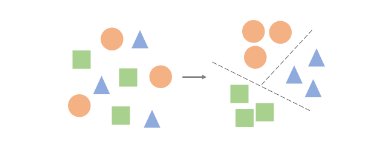
\includegraphics[width=1\textwidth]{imagenes/ml-supervised-learning.png}
    \end{center}
    \caption[Aprendizaje supervisado]{Figura extraída de \cite{sah2020machine} que muestra un ejemplo de aprendizaje supervisado.}
\end{figure}

\subsection{Aprendizaje no supervisado}
Cuando los datos solo vienen en forma de entrada y no se tiene ninguna salida (no hay etiquetas) entonces se trata de un aprendizaje no supervisado. Los algoritmos de este tipo se basan en la diferenciación de los datos mediante los patrones subyacentes que puedan encontrar. Son comunes en el aprendizaje no supervisado los algoritmos de \textit{clustering}~\cite{sah2020machine}.

\begin{figure}[htp]
    \begin{center}
        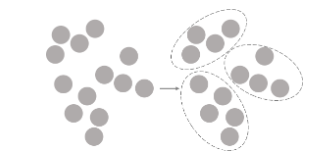
\includegraphics[width=0.7\textwidth]{imagenes/ml_unsupervised-learning.png}
    \end{center}
    \caption[Aprendizaje no supervisado]{Figura extraída de \cite{sah2020machine} que muestra un ejemplo de aprendizaje no supervisado. Se trata de dividir en clústers sin información de etiquetas.}
\end{figure}

\subsection{SVM}
Las máquinas de vectores de soporte o \textit{SVM} fueron introducidas por primera vez en~\cite{cortes_support-vector_1995}. En este documento será uno de los algoritmos de clasificación usados en la función \textit{fitness} para cuantificar la calidad de los pesos aprendidos por los algoritmos optimizadores.\\[6pt]
Las máquinas de vectores de soporte son algoritmos cuya principal característica se basa en la creación de un hiperplano o conjunto de hiperplanos en un espacio $n$-dimensional~\cite{scikit-learn-svm,}. Este hiperplano o hiperplanos es elegido de manera que maximice el margen entre los puntos de datos de todas las clases a predecir. El margen es la distancia entre el hiperplano y los puntos de datos más cercanos de cada clase, estos puntos se denominan vectores de soporte. De esta manera se consigue minimizar el error de generalización~\cite{hastie2009elements}.\\[6pt]
La idea más intuitiva es, que al haber más espacio entre los puntos de distintas clases, hay más posibilidad de que los puntos no vistos, los puntos a predecir, caigan en zonas correctas. En este documento se utilizará este algoritmo como clasificador y se por ello referido como \textbf{SVC} (\textit{support vector classifier}).

\begin{figure}[htp]
    \begin{center}
        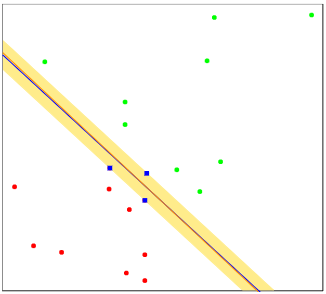
\includegraphics[width=0.5\textwidth]{imagenes/svm-margin.png}
    \end{center}
    \caption[Margen en SVM]{Figura extraída de \cite{hastie2009elements} en la que se muestra de forma gráfica en un espacio $2$-dimensional el margen óptimo de separación de dos clases.}
\end{figure}

\subsection{K-nearest neighbors}
El algoritmo de $k$ vecinos más cercanos fue presentado en \cite{fix_discriminatory_1989} por Evelyn Fix y Joseph Hodges, y más tarde ampliado en \cite{cover_nearest_1967} por Thomas Cover.\\[6pt]
Puede ser utilizado para regresión o clasificación, pero su uso suele darse más en este último problema. Este algoritmo ofrece una premisa sencilla, la clase de un punto $p$ dependerá de cuál sea la clase mayoritaria dentro del subconjunto de $k$ vecinos más cercanos~\cite{10.1007/978-3-540-39964-3_62}.\\[6pt]
El funcionamiento del algoritmo se puede resumir en los siguientes pasos:

\begin{enumerate}
    \item \textbf{Selección del valor de $k$}: El usuario debe determinar el número de vecinos a considerar. Este número puede variar dependiendo del problema y los datos específicos.

    \item \textbf{Cálculo de distancias}: Para un punto nuevo, se calculan las distancias a todos los puntos en el conjunto de datos de entrenamiento. Las distancias comúnmente se calculan utilizando métricas como la distancia euclidiana, aunque otras métricas (como la distancia de Manhattan o la distancia de Minkowski) pueden ser utilizadas dependiendo del contexto y las características de los datos.

    \item \textbf{Identificación de los $k$ vecinos más cercanos}: Una vez calculadas las distancias, se seleccionan los $k$ puntos del conjunto de datos de entrenamiento que estén más cerca del punto nuevo.

    \item \textbf{Asignación de clase (para clasificación)}: La clase del nuevo punto se determina por la mayoría de votos entre los $k$ vecinos seleccionados. En otras palabras, se asigna la clase más común entre estos vecinos.

    \item \textbf{Predicción de valor (para regresión)}: En el caso de la regresión, el valor predicho para el nuevo punto es el promedio (o alguna otra función agregada) de los valores de los $k$ vecinos seleccionados.
\end{enumerate}

Valores mayores de $k$ incrementan la varianza, pero decrementan el sesgo (equilibrio sesgo-varianza~\cite{Mostafa2012}). De forma inversa, a menor $k$ mayor sesgo y menor varianza.\\[6pt]
Otra forma de verlo es que si $k=1$ (el valor mínimo), el modelo entrenado será muy complejo, pues cada punto puede variar de clase por mínimo que sea el cambia en su entorno. Es un modelo que tiende a sobre-ajustar. Con $k=n$ el modelo es lo más simple posible, al tener en cuenta absolutamente todos los puntos, la clasificación será siempre la de la clase más repetida.